% *******************************************************************************
% * Copyright (c) 2007 by Elexis
% * All rights reserved. This document and the accompanying materials
% * are made available under the terms of the Eclipse Public License v1.0
% * which accompanies this distribution, and is available at
% * http://www.eclipse.org/legal/epl-v10.html
% *
% *  $Id: varianten.tex 2469 2007-06-02 19:47:42Z rgw_ch $
%
%*******************************************************************************
% !Mode:: "TeX:UTF-8" (encoding info for WinEdt)

\section{Le logiciel seul sous différentes Variantes}
\label{varianten}
AU début de ce livre (s. S. \pageref{easyinstall}) vous avez vu la simple installation de base. Si vous souhaitez mieux controler les fichier téléchargés et la configuration du logiciel, vous pouvez aussi télécharger des composantes spécifiques du logiciel. Dans la partie qui suit vous trouverez des explications concernant ce dont vous avez besoin.

Il est essentiel de vous rendre attentifs sur le fait que tous les fichiers téléchargeables créent une base de données vide qui n'est utilisable qu'après une installation et configuration de base qui elle-même n'est pas trop simple. Pour cette raison nous recommandons pour un essai plutôt l'installation standard.

\section{Differnts types d'installateur}
Elexis est basé sur un environnement \textit{Eclipse Rich Client} qui est lui-même basé sur \textit{Java Runtime Environment}, qui est basé sur le système d'exploitation de votre ordinateur. Aussi OpenOffice est intégré dans le système d'exploitation et coopère directement avec le Java Runtime de même qu'avec le système d'exploitation et Elexis. La figure suivante veut expliquer ce contexte:
\begin{figure}[hb]
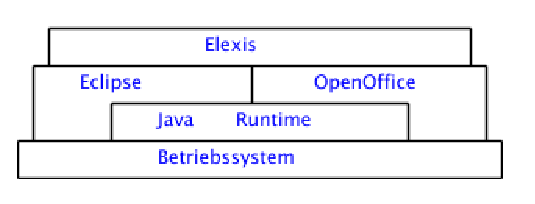
\includegraphics{images/modell}
\caption{Elexis Modell}
\label{Aufbau von Elexis}
\end{figure}

Dépendant de ce qui est déjà installé sur l'ordinateur on aura besoin d'un paquet plus ou moins volumineux.

\section{Paquet complet y inclus JRE (JAVA Runtime Environment)}

Utilisez ce paquet si vous n'avez pas de Java-Runtime sur votre système et si vous installez Elexis pour la première fois. Vous pouvez tester l'existence d'un Java-Runtime sur votre système de façon suivante : 

Ouvrez une ligne de commandement (dans Windows: cmd.exe, pour Mac et Linux: Terminal respct. xterm) introduisez:

\textit{java -version} \texttt{enter}

Si vous recevez maintenant un message d'erreur (commande ou fichier infrouvable) Java n'est pas ou pas correctement installé. Si vous recevez le message d'une version < 1.5, votre version Java est trop vieille. En ce cas vous avez besoin de ce paquet:
\begin{itemize}
 \item Installateur complet pour Windows:  \href{http://www.elexis.ch/download.php?file=demo} {elexis-win32-jre.exe}
\item Installateur complet pour Linux x86:  \href{http://www.elexis.ch/download.php?file=elexis-linux-jre-i386}{elexis-linux.i386-jre.run}


\end{itemize}


Commentaire
L'installation ne provoquera (à part de l'utilisation de ~50 MO) aucun autre changement dans votre cordinateur. De même, l'installation du Java Runtime ne se fera que localement dans le répertoire de Elexis et peut facilement être supprimée avec celui.
%
%hier fehlen noch die url
%
\subsection{Paquet complet sans JRE}
Utilisez ce paquet lorsque vous avez installé un Java Runtime sur votre système et vous souhaitez installer Elexis pour la première fois
\begin{itemize}
 \item Installateur pour Windows:  \href{http://www.rgw.ch/download.php?file=elexis-win32}{elexis-win32.exe}
\item Installateur pour Linux x86:  \href{http://www.elexis.ch/download.php?file=elexis-linux-i386}{elexis-linux-i386.run}
\item Archives pour MacOS X (10.4 ou plus): \href{http://www.elexis.ch/download.php?file=elexis-mac}{Installer, ca. 25MB}
\end{itemize}

\subsection{Plugin seul}
Ceci vous nécessitez si vous avez déjà installé Elexis et si vous souhaitez installer une nouvelle version. Le plugin est pour tous les systèmes d'exploitation le même, raison pour laquelle il n'y a qu'un seul fichier.
\begin{itemize}
 \item Tous les systèmes :  \href{http://www.elexis.ch/download.php?file=elexis-plugin}{elexis-plugin.zip, ca. 5MB}
\item \href{http://www.elexis.ch/download.php?file=demodaten.zip}{Demo-Datenbank, ca. 12MB}
\end{itemize}

\subsection{version démo de la base de données}
Si vous souhaitez tester Elexis sans configuration veuillez télécharger la base de donnée version démo (~11 MO). Décompressez le fichier .zip dans votre dossier Elexis (de sorte qu'on trouvera dans le dossier Elexis un sous-dossier \textit{Plugins}, \textit{Con\-figu\-ra\-tion}, éventuellement \textit{work\-space}
et en plus \textit{demoDB}, à part des fichiers Elexis.exe, Elexis.ini et autres.

Indépendamment d'un règlage quelconque, Elexis accède que sur cette base de données s'il trouve lors du démarrage un dossier demoDB dans son répertoire. Si vous voulez plus tard accéder à une autre base de données, il faudra effacer ou renommer le dossier \textit{demDB}.

Pour le login d'un utilisateur dans la base de données demoDB veuillez introduire comme nom et mot de passe \textit{test}(sans guillemet), le compte de l'administrateu porte le nom Administrator et le mot de passe est : admin.
\section{Downloads}
Vous trouvez ici des différentes variantes du fichier. Vous trouverez à la page ellen des explications plus détaillées concernant la signification des différents fichiers }.
\subsection{Instructions imprimables pour le débutant}

\begin{itemize}
 \item \href{http://www.elexis.ch/files/erste_schritte.pdf}{Instructions pour l'installation et petit  manuel pour les premiers pas(PDF)}
\item \href{http://www.elexis.ch/files/pat_agenda.pdf}{Introduction saisie du patient et installation de l'agenda}
\end{itemize}

\subsection{Programme pour Microsoft Windows (2000, XP Home ou XP pro)}
\begin{itemize}
\item \href{http://www.elexis.ch/download.php?file=demo}{complet avec OpenOffice, données pour exemples Java (~150 MO)}
\item \href{http://www.rgw.ch/download.php?file=elexis-jre-win32}{Installateur avec Java runtime (~40MO)}
\item \href{http://www.rgw.ch/download.php?file=elexis-win32}{Installateur sans Java runtime ~20MO)}
\end{itemize}

\subsection{Programme pour Linux i386 (ou AMD64)}
\begin{itemize}
 \item \href{http://www.elexis.ch/download.php?file=elexis-linux-jre-i386}{Installateur avec Java runtime ( ~50 MO)}
\item \href{http://www.elexis.ch/download.php?file=elexis-linux-i386}{Installateur sans Java runtime (~30 M=)}
\end{itemize}

\subsection{Programme pour Apple Macintosh à partir de OSX 10.4 (Tiger)}
\begin{itemize}
 \item \href{http://www.elexis.ch/download.php?file=elexis-mac}{Installateur (~ 25MO)}
\end{itemize}

\subsection{Tout les systèmes:}
\begin{itemize}
 \item \href{http://www.elexis.ch/download.php?file=elexis-plugin}{Elexis-Plugin seul (~5MO)}
\item \href{http://www.elexis.ch/download.php?file=demodaten.zip}{base de données version démo  (~12MO) }
\end{itemize}

\subsection{données de base:}
\begin{itemize}
 \item \href{http://cug.zur-rose.ch/aerztegrossist/aerztegrossist.asp}{données de base des médicaments. (gratuit pour pour des clients de Apotheke zur Rose,  ASAS-Login)}
\item \href{http://www.polymed.ch/d/aktuell/downloads.html}{base de données articles de Polymed}
\item \href{http://www.tarmedsuisse.ch/fileadmin/media/Dateien/Browser/TARMED_Database_1.03.zip}{base de données Tarmed}
\item \href{http://www.dimdi.de/dynamic/de/klassi/downloadcenter/icd-10-gm/version2006/systematik/x1gea2006.zip}{ICD-10}
\item \href{http://www.famh.ch/liste_analyses_d_06.pdf}{liste des analyses (accessible qu'en format PDF )}
\item \href{http://www.bag.admin.ch/themen/krankenversicherung/02874/index.html?lang=de&download=M3wBUQCu/8ulmKDu36WenojQ1NTTjaXZnqWfVpzLhmfhnapmmc7Zi6rZnqCkkIV6e3l9bKbXrZ2lhtTN34al3p6YrY7P1oah162apo3X1cjYh2+hoJVn6w==}{MiGeL (que PDF)}
\end{itemize}

